\documentclass[12pt,a4paper]{article}

\usepackage{fontspec}
\usepackage{polyglossia}
\setdefaultlanguage{russian}
\setotherlanguage{english}

\setmainfont{Arial}
\setsansfont{Arial}
\setmonofont{Courier New}
\newfontfamily\cyrillicfont{Arial}
\newfontfamily\cyrillicfontsf{Arial}
\newfontfamily\cyrillicfonttt{Courier New}

\usepackage{geometry}
\geometry{margin=2.5cm}

\usepackage{graphicx}
\usepackage{float}
\usepackage{booktabs}
\usepackage{tabularx}
\usepackage{array}
\usepackage{makecell}
\usepackage{hyperref}
\usepackage{needspace}
\hypersetup{hidelinks}

\setlength{\parindent}{1.25cm}
\setlength{\parskip}{0.35em}

\newcolumntype{Y}{>{\centering\arraybackslash}X}

\newcommand{\punkt}[2]{\Needspace{4\baselineskip}\noindent\textbf{#1.} #2\par}

\title{Лабораторная работа\\"Визуализация магнитных полей"}
\author{}
\date{}

\begin{document}
\maketitle

\section*{Теоретические сведения}

\textbf{1. Магнитное поле прямого проводника и зависимость от расстояния.}
Для длинного прямого проводника с током модуль магнитной индукции убывает обратно пропорционально расстоянию $r$:

\[
B(r) = \frac{\mu_0 \mu I}{2\pi r}.
\]

Величина напряженности магнитного поля равна

\[
H(r) = \frac{I}{2\pi r},
\]

а связь между $B$ и $H$ в среде:

\[
B = \mu_0 \mu_r H.
\]

В вакууме $\mu_r = 1$, поэтому $B = \mu_0 H$.

\textbf{2. Равновесная точка двух параллельных проводников.}
При сонаправленных токах между проводниками существует точка, где поля компенсируются:

\[
\frac{\mu_0 \mu I_1}{2\pi r_1} = \frac{\mu_0 \mu I_2}{2\pi r_2}
\quad \Rightarrow \quad
\frac{I_1}{r_1} = \frac{I_2}{r_2},
\]

при геометрическом ограничении $r_1 + r_2 = d$.

\textbf{3. Принцип суперпозиции магнитных полей.}
Поле в точке от нескольких источников равно векторной сумме полей от каждого источника:

\[
\vec{B}_{\Sigma} = \sum\limits_{k=1}^{n} \vec{B}_k.
\]

\textbf{4. Распределение поля системы параллельных проводников.}
Карта поля формируется суперпозицией вкладов всех проводников; изменение направлений токов меняет направление векторов $B_k$, а изменение силы токов меняет их модуль.

\clearpage

\section*{Практическая часть (эксперименты)}

\subsection*{Эксперимент 1. Экспериментальное определение степени зависимости величины вектора магнитного поля от расстояния до источника}

\punkt{1}{В программе \texttt{MagneticFieldVisualization.exe}, используя правую панель, создать линейный проводник в плоскости экрана, проходящий через две заданные точки так, чтобы он располагался параллельно одной из осей координат.}

\begin{figure}[H]
    \centering
    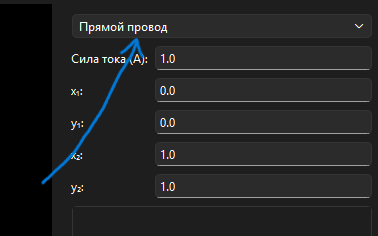
\includegraphics[width=0.4\linewidth]{images/add_panel.png}
\end{figure}

\begin{figure}[H]
    \centering
    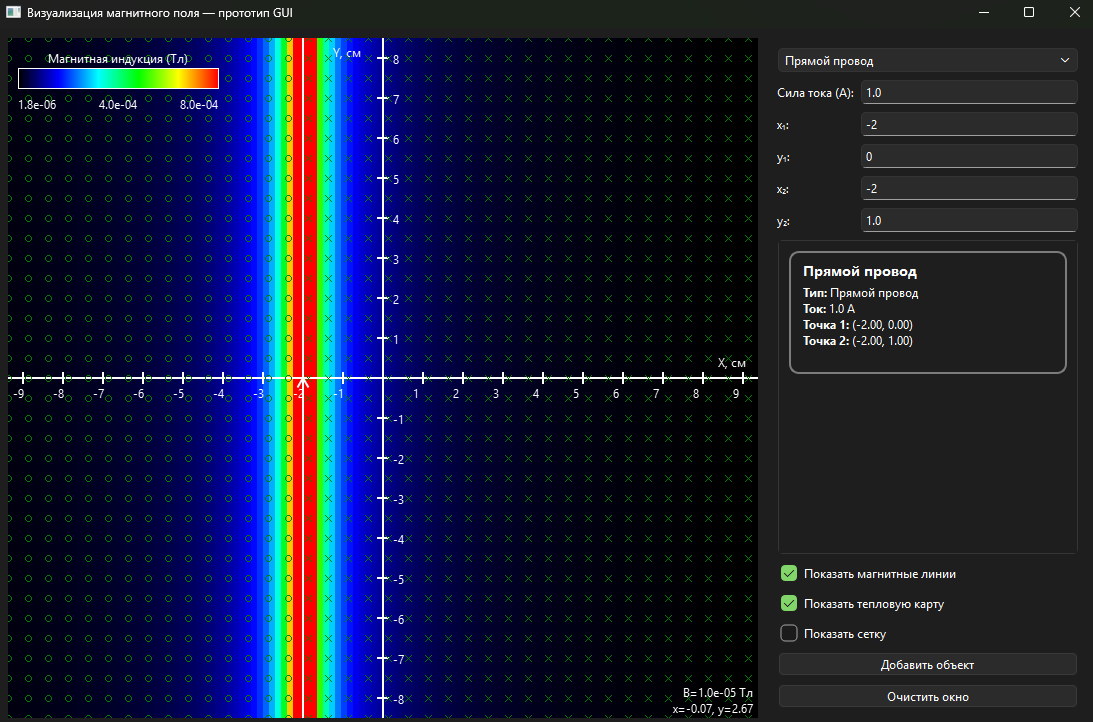
\includegraphics[width=1.1\linewidth]{images/linear_conductor.png}
\end{figure}

\begin{quote}
Если подвести курсор к интересующей точке рабочей области, в правом нижнем углу экрана появится информация о точной координате курсора и величине магнитного поля под ним.
\end{quote}

\punkt{2}{Используя курсор, определить величину магнитного поля на расстоянии 1 см от проводника. Записать значение магнитного поля в таблицу:}

\begin{table}[H]
    \centering
    \small
    \setlength{\tabcolsep}{4pt}
    \renewcommand{\arraystretch}{1.2}
    \begin{tabular}{|c|c|c|c|c|}
        \hline
        \makecell{Номер\\измерения $N$} & \makecell{Расстояние до\\проводника $L_n$} & \makecell{Индукция\\магнитного поля $B_n$} & \makecell{Кратность\\$L_i/L_{i-1}$} & \makecell{Кратность\\$B_i/B_{i-1}$} \\
        \hline
        1 &  &  & X & X \\
        \hline
        2 &  &  &  &  \\
        \hline
        3 &  &  &  &  \\
        \hline
        4 &  &  &  &  \\
        \hline
    \end{tabular}
\end{table}

\begin{figure}[H]
    \centering
    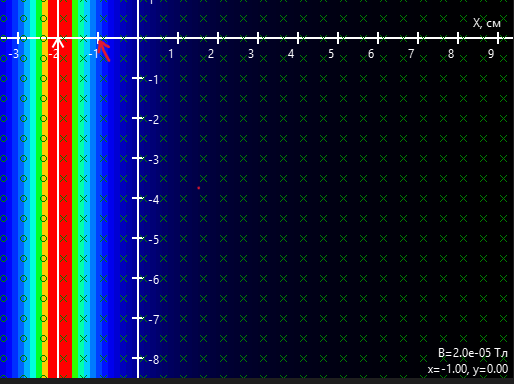
\includegraphics[width=0.9\linewidth]{images/1cm_point.png}
\end{figure}

\punkt{3}{Аналогичным образом определить магнитное поле на расстоянии 2 см и 4 см и так далее. Сравнить полученные результаты. Сделать выводы о характере зависимости величины индукции магнитного поля от расстояния до источника магнитного поля.}

\begin{table}[H]
    \centering
    \small
    \setlength{\tabcolsep}{4pt}
    \renewcommand{\arraystretch}{1.2}
    \begin{tabular}{|c|c|c|c|c|}
        \hline
        \makecell{Номер\\измерения $N$} & \makecell{Расстояние до\\проводника $L_n$} & \makecell{Индукция\\магнитного поля $B_n$} & \makecell{Кратность\\$L_{i+1}/L_i$} & \makecell{Кратность\\$B_{i+1}/B_i$} \\
        \hline
        1 & 1 см & $2.0 \times 10^{-5}$ & X & X \\
        \hline
        2 & 2 см & $1.0 \times 10^{-5}$ & 2 & $1/2$ \\
        \hline
        3 & 4 см & $5.0 \times 10^{-6}$ & 2 & $1/2$ \\
        \hline
        4 & 6 см & $3.3 \times 10^{-6}$ & 1.5 & $2/3$ \\
        \hline
    \end{tabular}
\end{table}

\textbf{Вывод:} При увеличении расстояния в $K$ раз магнитная индукция (и напряженность магнитного поля) уменьшается в $K$ раз, что согласуется с зависимостью $B \sim \frac{1}{r}$.

\clearpage

\subsection*{Эксперимент 2. Нахождение равновесной точки двух источников магнитного поля}

\punkt{1}{Создать два параллельных проводника на расстоянии 6 см. Сила тока одного из них $I_1 = 1$ А, другого $I_2 = 2$ А. Токи сонаправлены.}

\begin{figure}[H]
    \centering
    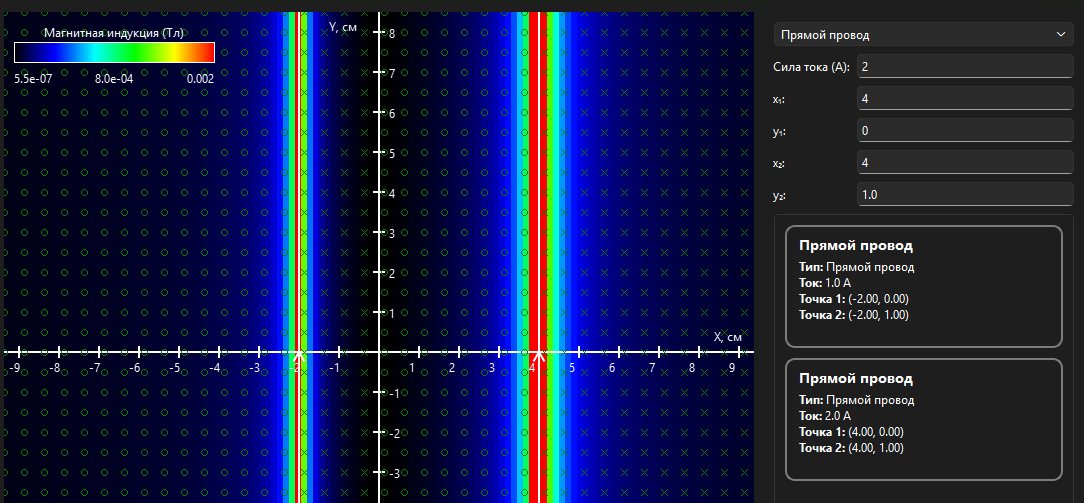
\includegraphics[width=0.9\linewidth]{images/two_conductors.png}
\end{figure}

\punkt{2}{Экспериментально определить расстояние, на котором поля от проводников будут компенсироваться. Обратить внимание на соотношение расстояний.}

\punkt{3}{Проверить аналитически:}


\[
\frac{\mu_0 I}{2\pi R_1} = \frac{\mu_0 2I}{2\pi R_2}
\]

\textbf{Повторить для других произвольных значений и направлений тока (с учетом знака). Сделать вывод.}


\begin{quote}
Вывод: расстояния $R_1/R_2$ соотносятся как $I_1/I_2$.
\end{quote}

\clearpage

\subsection*{Эксперимент 3. Экспериментальная проверка выполнимости принципа суперпозиции магнитных полей}

\punkt{1}{Используя произвольное количество (от 3-х) проводников, находящихся в плоскости рисунка (не "Провод-точка"), определить характеристику поля, создаваемого ими по отдельности в одной выбранной точке пространства.}

\punkt{2}{Установить все источники одновременно и определить интенсивность поля в этой точке. Убедиться в выполнимости принципа суперпозиции в любой точке пространства.}

\begin{figure}[H]
    \centering
    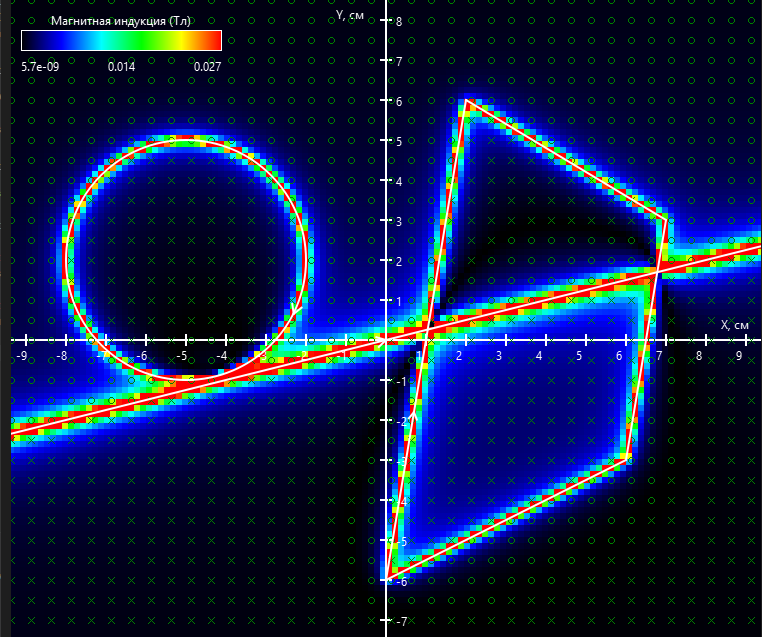
\includegraphics[width=0.9\linewidth]{images/several_sources.png}
\end{figure}

\clearpage

\subsection*{Эксперимент 4. Наблюдение распределения напряженности магнитного поля среди сложной конфигурации параллельных проводников}

\punkt{1}{Расставить произвольное количество проводников, перпендикулярных плоскости рисунка ("Провод-точка"). Поэкспериментировать с направлением и силой тока.}

\punkt{2}{Убедиться в вихревом характере силовых линий магнитного поля.}

\begin{figure}[H]
    \centering
    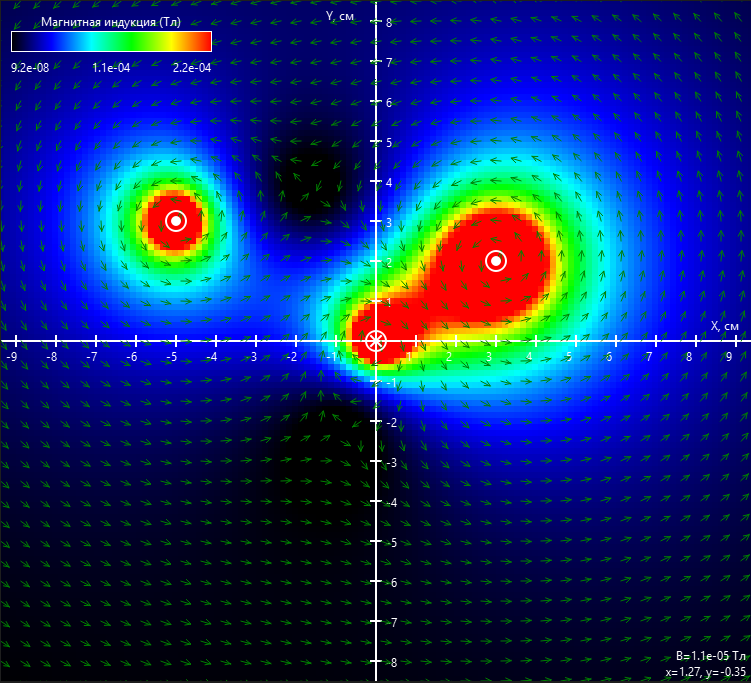
\includegraphics[width=0.9\linewidth]{images/picture_1.png}
\end{figure}

\begin{figure}[H]
    \centering
    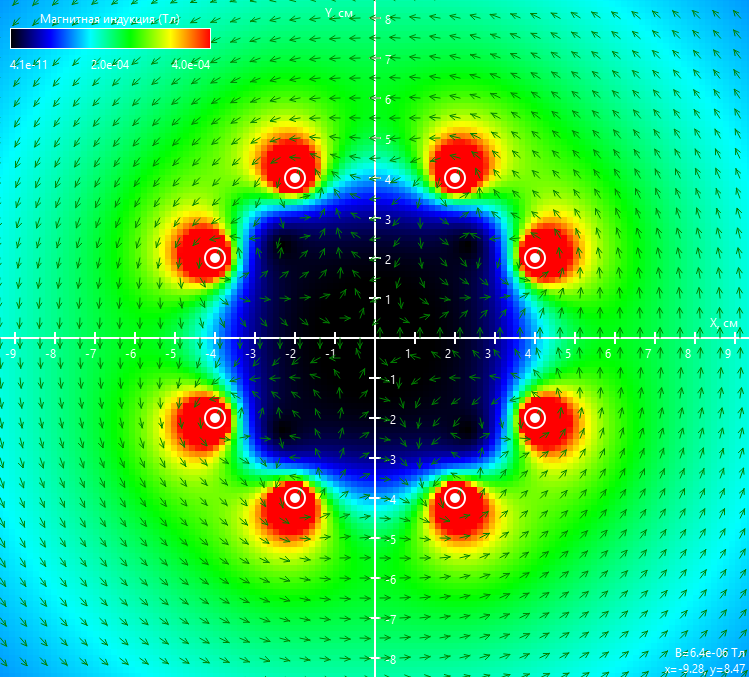
\includegraphics[width=0.9\linewidth]{images/picture_2.png}
\end{figure}

\begin{figure}[H]
    \centering
    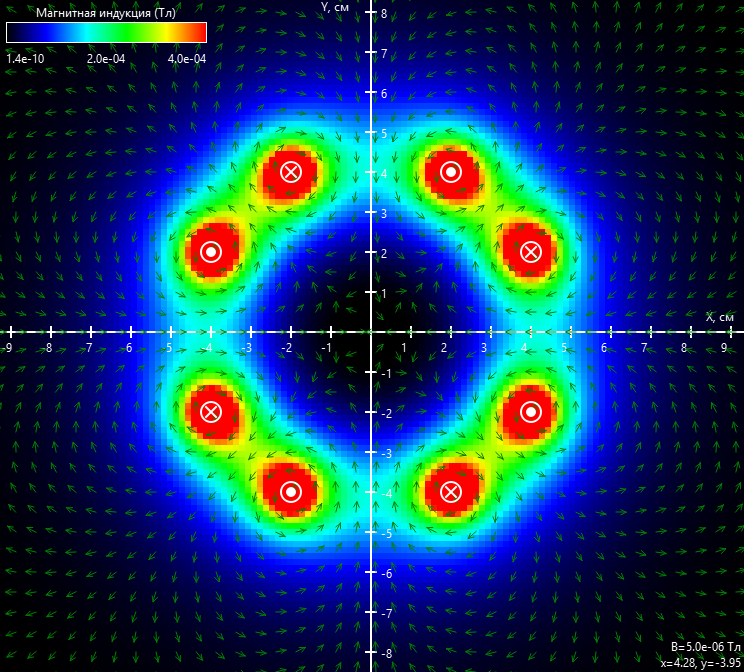
\includegraphics[width=0.9\linewidth]{images/picture_3.png}
\end{figure}

\begin{figure}[H]
    \centering
    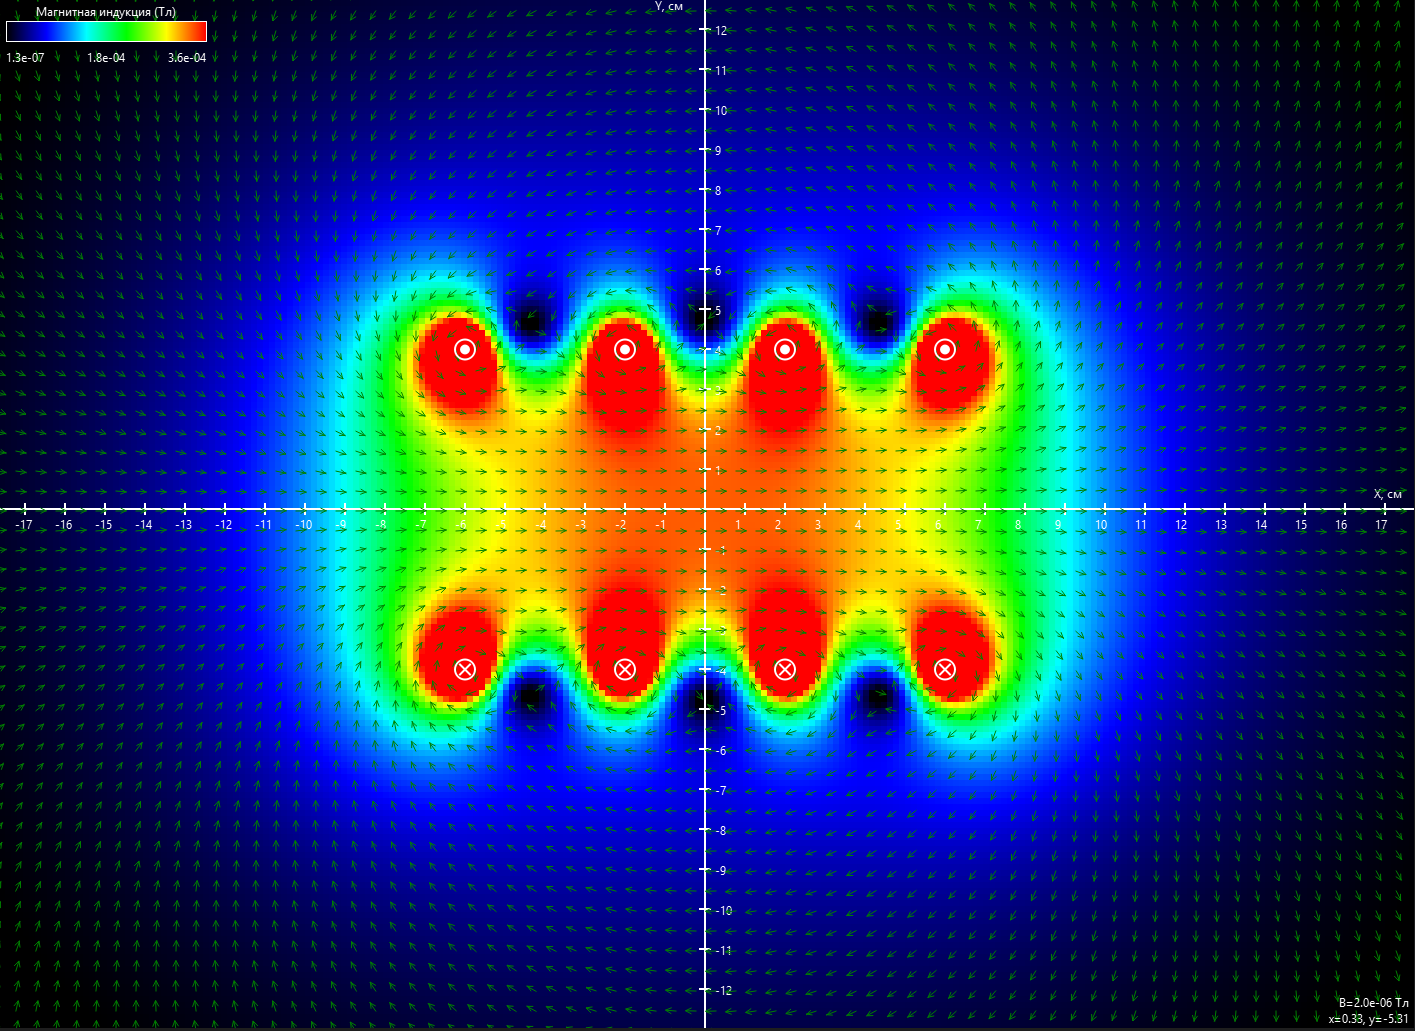
\includegraphics[width=0.9\linewidth]{images/picture_4.png}
\end{figure}

\end{document}
